\section{Methods}
\label{section:methods}

As in the case of Scene Text Detection / Recognition, it is effective to separate Text Detection
and Text Recognition and treat them as different problems.
Furthermore, it is possible to record the written area due to the characteristics of the electronic tablet,
so using a simple heuristic on the trajectory data eliminates the need to actually perform text detection.
The role of this step, namely "Region of Interest Detection" step is to reduce the size of data
passed to the subsequent processing and suppress the increase in the amount of calculation.
Detected regions are then preprocessed and passed to the text recognition module. In the text recognition module,
two patterns of recognition using CTC and recognition using the API provided by Apple were verified.

\subsection{Region of Interest Detection}

The purpose of Region of Interest (ROI) detection is to cut out sub-sequence
representing words and illustrations from the dot sequence of the pen tip trajectory
and cut back the data to be passed to the subsequent processing to
reduce the amount of calculation and improve the recognition accuracy.
Region of interest is a region including a dot sequence of the word or the illustration.
To specify the region, two assumptions are made on region of interest.

\begin{enumerate}
    \item Objects drawn in the region of interest are close in time when drawn
    \item Objects drawn in the region of interest are spatially close
\end{enumerate}

Based on these assumptions, ROI is detected by the following algorithm \ref{alg:roi}.
Then the smallest rectangle containing the obtained point sequence is the ROI.
It should be noted that we prioritize the reduction of the amount of computation and
terminate the search for subsequences on the way.As a result, points that are not continuous
in time but close in space may not be included in the ROI depending on the threshold setting.
However, when priority is given to spatial proximity, it is necessary to parse the entire
trajectory every time we perform ROI detection, and if the size of the point sequence becomes large,
it may be a bottleneck in calculation. Therefore we decided to use this method,
but better approaches will be discussed in the section \ref{section:conclusion}.

\begin{algorithm}
\DontPrintSemicolon
    \KwInput{$S=\{s_1,s_2,\cdots,s_n\}~where~s_i=(c_i, t_i)$}
    \KwOutput{$\sigma=\{s_k, s_k+1, \cdots, s_n\}~1\le k \le n$}
    subset := \{\} \\
    $c_{prev} := c_n$ \\
    $t_{prev} := t_n$ \\
    \For{$s_i~in~reversed(S)\setminus s_n$}
    {
        $c_i, t_i \leftarrow s_i$\\
        \If{$t_{prev} - t_i < t_{threshold}$}
        {
            $subset \leftarrow subset \cup \{s_i\}$ \\

        } \Else{
            \If{$distance(c_{prev}, c_i) < c_{threshold}$}{
                $subset \leftarrow subset \cup \{s_i\}$
            } \Else {
                break
            }
        }
        $c_{prev} \leftarrow c_i$ \\
        $t_{prev} \leftarrow t_i$
    }
\caption{ROI detection}
\label{alg:roi}
\end{algorithm}

Figure \ref{fig:region_of_interest} shows an example of the region detected with
this heuristic.

There are some cases where such heuristics do not work. For example, when the scale of
the depicted object is large, the gap between the sequence of points
constituting the object may be too large and fail.It is also a major problem that
temporal and spatial proximity depends on parameters and sometimes does not match intuition.
However, it is certain that this method can narrow down the target area for text recognition
with a very small amount of computation, so this report adopted this method.

\begin{figure}
    \centering
    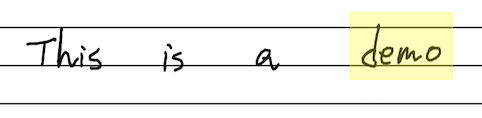
\includegraphics[width=\linewidth]{images/region_of_interest.png}
    \caption{The region with yellow overlay is detected region of interest}
    \label{fig:region_of_interest}
\end{figure}

\subsection{Recognition}

In text recognition, two models were tried: a model that directly reads the content from the
result of region of interest detection using CTC, and the model which is provided by
Apple\footnote{https://developer.apple.com/documentation/vision/vnrecognizetextrequest}.
Note that Apple's VNRecognizeTextRequest API does not disclose its implementation or
the model used inside, it is unknown exactly what processing is being done.

\subsubsection{CTC}

CTC models are usually constructed using CNN model with Recurrent Neural Network (RNN)
as the output layer.
However, RNN performs computations slowly compared to CNN,
and in recent years its effectiveness in CTC is sometimes questioned~\cite{puigcerver2017multidimensional}.
Given that all calculations are done on iOS, and based on research that the
output layer of the CTC model can also be configured using CNN~\cite{gao2017reading}, in this report
a model which is fully constructed only by CNN was used for CTC model. The detail of the
model configuration can be found in the repository\footnote{https://github.com/koukyo1994/iOS-note-v2/blob/master/prototype/py/model.py}.
To get an approximation for most probable labeling, greedy policy, the policy to take the
most probable label at each time step, was used.

\subsubsection{VNRecognizeText API}
VNRecognizeText API is an API provided by Apple officially,
and its function is to detect text from the whole area where the drawing is and read it.
Therefore there's no need to detect the region of interest to read the content inside.
However, in order to make the inference fast, we used ROI detection as a preprocessing before
putting an image to the API.
This API is completely a black box, accepts an image of any shape as input,
reads the text in it, and outputs it with position information.

VNRecognizeText API has two modes for recognition, namely `.fast` and `.accurate`\footnote{https://developer.apple.com/documentation/vision/vnrequesttextrecognitionlevel}.
According to the official introduction video\footnote{https://developer.apple.com/videos/play/wwdc2019/234/}
if VNRecognizeText API, `.fast` uses traditional feature based method inside while
`.accurate` uses more sophisticated Computer Vision model inside. As the names of those imply
`.fast` is faster but not so accurate while `.accurate` is slower but more accurate. Both `.fast` and `.accurate`
were tested. However, since `.fast` failed to recognize any handwritten letters, measurement on `.fast` was not conducted.
\subsection{Auto-Complete}

In this report, we deal with auto-completion as an application of the inference result.
This auto-completion emphasizes simplicity and presents words
that start with infered result in order of frequency. To get the word candidates
which start with infered result, we created an inverse index
that maps the first few letters of words to a group of words with that prefix.
For example, index "elbo" corresponds to word group \{"elbow", "elbow's", "elbowed", "elbowing", "elbowroom", "elbowroom's", "elbows"\}.
Word suggestions for auto-completion are from `wamerican` package\footnote{https://packages.debian.org/search?keywords=wamerican} of Debian GNU/Linux.
Word frequencies were counted using wikipedia-word-frequency\footnote{https://github.com/IlyaSemenov/wikipedia-word-frequency}.
We implemented auto-completion to be performed each time the pen is released from the tablet surface.

\subsection{Dataset}

Handwritten character recognition and handwritten sentence recognition are
fields that have been studied for a long time, so there are many data sets,
but these are often provided in different formats, and there is some difficulty
in eliminating differences between formats and using them for training dataset.
We therefore took an approach to create a composite dataset by
embedding a combination of existing handwritten-like fonts with randomly picked fontsize and
randomly selected English words in the image. The words are selected from `wamerican` package
and 10,000 images were generated for training. We split the dataset to 80\% / 20\% each for training / validation.
The fonts used are listed up in the repository\footnote{https://github.com/koukyo1994/iOS-note-v2/blob/master/prototype/py/fonts/list.txt}.
Figure \ref{fig:generated_image} shows an example of training data generated with this method.

\begin{figure}
    \centering
    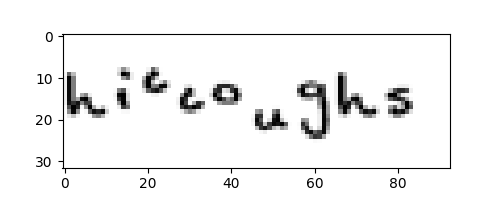
\includegraphics[width=\linewidth]{images/generated_image.png}
    \caption{Generated image using handwritten-like fonts}
    \label{fig:generated_image}
\end{figure}

For image pre-processing, we only used vertical and horizontal random offset of characters in a word.
Since the image taken from the prototype application has white background with no blurriness,
we didn't apply further image augmentation techniques.

\subsection{Implementation}

We used Python3.6\footnote{https://www.python.org/downloads/release/python-360/} and
TensorFlow2.1\footnote{https://www.tensorflow.org/} for building machine learning
models and training, and used coremltools3.2\footnote{https://apple.github.io/coremltools/}
to convert the models into the format that can work on iOS.For training,
Adam optimizer with learning rate 5e-5. `beta\_1` and `beta\_2` parameters are set to 0.9 and 0.999 each.
The trainig was performed 50 epochs with batch size 32.

To get handwritten document image from the iOS electronic tablet, a function to print
the input from the Apple Pencil\footnote{https://www.apple.com/apple-pencil/} on the white canvas
according to the path of the pen has been implemented.

For training the model, Google Colaboratory environment
\footnote{https://colab.research.google.com/notebooks/welcome.ipynb} has been used.
All the implementation is published at the GitHub repository\footnote{https://github.com/koukyo1994/iOS-note-v2}.
